%%%%%%%%%%%%%%%%%%%%%%%%%%%%%%%%%%%%%%%%%%%%%%%%%%%%%%%%%%%%%%%%%%%%%%%%
% Uni Duesseldorf
% Lehrstuhl fuer Datenbanken und Informationssysteme
% Vorlage fuer Bachelor-/Masterarbeiten
% Optimiert fuer den Original-Latex-Kompiler LATEX.EXE (LaTeX=>PS=>PDF)
%%%%%%%%%%%%%%%%%%%%%%%%%%%%%%%%%%%%%%%%%%%%%%%%%%%%%%%%%%%%%%%%%%%%%%%%
% Ueberarbeitung für pdflatex (LaTeX=>PDF)
%%%%%%%%%%%%%%%%%%%%%%%%%%%%%%%%%%%%%%%%%%%%%%%%%%%%%%%%%%%%%%%%%%%%%%%%
% Vorlage Changelog:
% 10.09.2015 (Matthias Liebeck): Nummerierung des Inhaltsverzeichnis nun römisch, Beispiel für einen Anhang eingebaut, \raggedbottom hinter sections eingefügt
% 11.07.2018 (Matthias Liebeck): Ersetzung des Bibliographiestils, Einsatz von Biber
% 04.09.2018 (Matthias Liebeck):
%   * Bibtex: unnötige Bibtexfelder beim Rendern ausblenden (thx @ Markus Brenneis)
%   * ngerman: "et al." im BibTeX für drei oder mehr Autoren
%   * Neuer Befehl \sectionforcestartright: Sections immer rechts beginnen (thx @ Philipp Grawe)
%   * ngerman: Deutsche Anführungszeichen im Literaturverzeichnis (thx @ Markus Brenneis)
%   * ngerman: Deutsche Anführungszeichen im Literaturverzeichnis (thx @ Markus Brenneis)
% 16.10.2018 (Matthias Liebeck): Zwei fixes an \sectionforcestartright (thx @ Markus Brenneis)
%%%%%%%%%%%%%%%%%%%%%%%%%%%%%%%%%%%%%%%%%%%%%%%%%%%%%%%%%%%%%%%%%%%%%%%%
%%%% BEGINN EINSTELLUNG FUER DIE ARBEIT. UNBEDINGT ERFORDERLICH! %%%%%%%
%%%%%%%%%%%%%%%%%%%%%%%%%%%%%%%%%%%%%%%%%%%%%%%%%%%%%%%%%%%%%%%%%%%%%%%%
% Geben Sie Ihren Namen hier an:

\newcommand{\bearbeiter}{Timo Stroick}

% Geben Sie hier den Titel Ihrer Arbeit an:
\newcommand{\titel}{Extraktion und Erweiterung eines Knowledge Graphen für Publikationen und Zitationen}

% Geben Sie das Datum des Beginns und Ende der Bachelorarbeit ein:
\newcommand{\beginndatum}{17. Juli 2020}
\newcommand{\abgabedatum}{19.~Oktober~2020}

% Geben Sie die Namen des Erst- und Zweitgutachters an:
\newcommand{\erstgutachter}{Prof. Dr.~Stefan Conrad}
\newcommand{\zweitgutachter}{Prof. Dr.~Michael Leuschel}

% Falls Sie die Arbeit zweiseitig ausdrucken wollen,
% benutzen Sie die folgende Zeile mit
% \AN fuer zweiseitigen Druck
% \AUS fuer einseitigen Druck
\newcommand{\zweiseitig}{\AN}
% true fuer biber, false fuer klassischen Zitierstil
%\newcommand{\biber}{false}
\newcommand{\biber}{true}

% Falls Sections immer rechts beginnen sollen. Gerade für Masterarbeiten
% interessant. Bei kurzen Bachelorarbeiten eher weniger zu verwenden.
\newcommand{\sectionforcestartright}{false}
%\newcommand{\sectionforcestartright}{true}

% Falls die Arbeit in englischer Sprache verfasst
% werden soll, dann benutzen Sie die folgende Zeile mit
% englisch fuer englische Sprache
% deutsch fuer deutsche Sprache
\newcommand{\sprache}{deutsch}

% Hier wird eingestellt, ob es sich bei der Arbeit um eine Bachelor
\newcommand{\arbeit}{Bachelorarbeit}

%%%%%%%%%%%%%%%%%%%%%%%%%%%%%%%%%%%%%%%%%%%%%%%%%%%%%%%%%%%%%%%%%%%%%%%%
%%%% ENDE EINSTELLUNGEN %%%%%%%%%%%%%%%%%%%%%%%%%%%%%%%%%%%%%%%%%%%%%%%%
%%%%%%%%%%%%%%%%%%%%%%%%%%%%%%%%%%%%%%%%%%%%%%%%%%%%%%%%%%%%%%%%%%%%%%%%

% Die folgende Zeile NICHT EDITIEREN oder loeschen


%%%%%%%%%%%%%%%%%%%%%%%%%%%%%%%%%%%%%%%%%%%%%%%%%%%%%%%%%%%
% Obere Titelmakros. Editieren Sie diese Datei nur, wenn
% Sie sich ABSOLUT sicher sind, was Sie da tun!!!
% (Z.B. zum Abaendern der BA-Vorlage in eine MA-Vorlage)
% Uni Duesseldorf
% Lehrstuhl fuer Datenbanken und Informationssysteme
% Version 2.2 - 2.3.2010
%%%%%%%%%%%%%%%%%%%%%%%%%%%%%%%%%%%%%%%%%%%%%%%%%%%%%%%%%%%
\newcommand{\AN}{twoside}
\newcommand{\AUS}{}


%\newcommand{\englisch}{}
%\newcommand{\deutsch}{\usepackage[german]{babel}}

%% Die folgenden auskommentierten Optionen dienen der automatischen
%% Erkennung des Latex-Kompilers und dem Setzen der davon abhängigen
%% Einstellungen. Bei Problem z.B. mit dem Einbinden von verschiedenen
%% Grafiktypen bei Verwendung von PdfLatex oder Latex, einfach die
%% verschiedenen \usepackage(s) ausprobieren. (Mit diesen Einstellungen
%% funktionierte diese Vorlage bei der Verwenundg von latex.exe als
%% Kompiler bei den meisten Studierenden.)

%\newif\ifpdf \ifx\pdfoutput\undefined
%\pdffalse % we are not running pdflatex
%\else
%\pdfoutput=1 % we are running pdflatex
%\pdfcompresslevel=9 % compression level for text and image;
%\pdftrue \fi

\documentclass[11pt,a4paper, \zweiseitig]{article}
\usepackage{ifthen}


%\usepackage[iso]{umlaute}
\usepackage[utf8]{inputenc}
\usepackage{palatino} % palatino Schriftart
%\usepackage{makeidx} % um ein Index zu erstellen
\usepackage[nottoc]{tocbibind}
\usepackage[T1]{fontenc} %fuer richtige Trennung bei Umlauten
\usepackage{fancybox} % fuer die Rahmen
\usepackage{shortvrb}
\usepackage{url}
\usepackage{xcolor}
\usepackage[colorlinks,citecolor=blue,linkcolor=black]{hyperref} %anklickbares Inhaltsverzeichnis

\ifthenelse{\boolean{\biber}}{
  % only needed for biber
  \usepackage[style=authoryear,natbib=true,backend=biber,mincitenames=1,maxcitenames=2,maxbibnames=99,uniquelist=false,dashed=false]{biblatex}

  % https://tex.stackexchange.com/a/334703/8850
  \AtEveryBibitem{%
    \clearfield{issn}
    \clearfield{isbn}
    \clearfield{doi}
    \clearfield{location}
    \clearlist{location}
    \clearlist{address}

    \ifentrytype{online}{}{% Remove url except for @online
      \clearfield{url}
    }
  }
}
{}%no else

% Falls es bei \citet ein Komma zwischen Name und Jahr gibt:
% https://tex.stackexchange.com/questions/312539/unwanted-comma-between-author-and-year-using-citet-command
% (thx @ Markus Brenneis)
%\DeclareDelimFormat[cbx@textcite]{nameyeardelim}{\addspace}



\ifthenelse{\equal{\sprache}{deutsch}}{
  \usepackage[ngerman]{babel}
  % Bibtex u.a -> et al.
  \ifthenelse{\boolean{\biber}}{
    \DefineBibliographyStrings{ngerman}{
      andothers = {{et\,al\adddot}},
    }
    \newcommand{\references}{Literatur}
  }
  {} % do nothing when not using biber
  \usepackage[autostyle, german=quotes]{csquotes} % Deutsche Anführungszeichen im Literaturverzeichnis (thx @ Markus Brenneis)

}{ \newcommand{\references}{References}}

\usepackage{a4wide} % ganze A4 Weite verwenden



%\ifpdf
%\usepackage[pdftex,xdvi]{graphicx}
%\usepackage{thumbpdf} %thumbs fuer Pdf
%\usepackage[pdfstartview=FitV]{hyperref} %anklickbares Inhaltsverzeichnis
%\else
%\usepackage[dvips,xdvi]{graphicx}
\usepackage{graphicx}
\usepackage{ulem}

%\fi

\newcommand{\redt}[1] {
  \textcolor{red}{#1}}

\newcommand{\oranget}[1] {
  \textcolor{orange}{#1}}

\newcommand{\purplet}[1] {
  \textcolor{purple}{#1}}

%%%%%%%%%%%%%%%%%%%%%%% Massangaben fuer die Arbeit %%%%%%%%%%%%%%%
\setlength{\textwidth}{15cm}

\setlength{\oddsidemargin}{35mm}
\setlength{\evensidemargin}{25mm}

\addtolength{\oddsidemargin}{-1in}
\addtolength{\evensidemargin}{-1in}

\ifthenelse{\boolean{\biber}}{\addbibresource{references.bib}}{}

%\makeindex
\begin{document}
%\setcounter{secnumdepth}{4} %Nummerieren bis in die 4. Ebene
%\setcounter{tocdepth}{4} %Inhaltsverzeichnis bis zur 4. Ebene

\pagestyle{headings}

\sloppy % LaTeX ist dann nicht so streng mit der Silbentrennung
%~ \MakeShortVerb{\§}

\parindent0mm
\parskip0.5em


{
\textwidth170mm
\oddsidemargin30mm
\evensidemargin30mm
\addtolength{\oddsidemargin}{-1in}
\addtolength{\evensidemargin}{-1in}

\parskip0pt plus2pt

% Die Raender muessen eventuell fuer jeden Drucker individuell eingestellt
% werden. Dazu sind die Werte fuer die Abstaende `\oben' und `\links' zu
% aendern, die von mir auf jeweils 0mm eingestellt wurden.

%\newlength{\links} \setlength{\links}{10mm}  % hier abzuaendern
%\addtolength{\oddsidemargin}{\links}
%\addtolength{\evensidemargin}{\links}

\begin{titlepage}
\vspace*{-1.5cm}
\raisebox{17mm}{
    \begin{minipage}[t]{70mm}
        \begin{center}
            %\selectlanguage{german}
            {\Large INSTITUT FÜR INFORMATIK\\}
            {\normalsize
                Datenbanken und Informationssysteme\\
            }
            \vspace{3mm}
            {\small Universitätsstr. 1 \hspace{5ex} D--40225 Düsseldorf\\}
        \end{center}
    \end{minipage}
}
\hfill
\raisebox{7mm}{
    
\includegraphics[width=130pt]{bilder/HHU_Logo}}
\vspace{14em}

% Titel
\begin{center}
    \baselineskip=55pt
    \textbf{\huge \titel}
    \baselineskip=0 pt
\end{center}

%\vspace{7em}

\vfill

% Autor
\begin{center}
    \textbf{\Large
        \bearbeiter
    }
\end{center}

\vspace{35mm}

% Prüfungsordnungs-Angaben
\begin{center}
%\selectlanguage{german}

%%%%%%%%%%%%%%%%%%%%%%%%%%%%%%%%%%%%%%%%%%%%%%%%%%%%%%%%%%%%%%%%%%%%%%%%%
% Ja, richtig, hier kann die BA-Vorlage zur MA-Vorlage gemacht werden...
% (nicht mehr nötig!)
%%%%%%%%%%%%%%%%%%%%%%%%%%%%%%%%%%%%%%%%%%%%%%%%%%%%%%%%%%%%%%%%%%%%%%%%%
{\Large \arbeit}

\vspace{2em}
\ifthenelse{\equal{\sprache}{deutsch}}{
    \begin{tabular}[t]{ll}
    Beginn der Arbeit:& \beginndatum \\
    Abgabe der Arbeit:& \abgabedatum \\
    Gutachter:         & \erstgutachter \\
    & \zweitgutachter \\
}{
    \begin{tabular}[t]{ll}
    Date of issue:& \beginndatum \\
    Date of submission:& \abgabedatum \\
    Reviewers:         & \erstgutachter \\
    & \zweitgutachter \\
}
\end{tabular}
\end{center}

\end{titlepage}

}

%%%%%%%%%%%%%%%%%%%%%%%%%%%%%%%%%%%%%%%%%%%%%%%%%%%%%%%%%%%%%%%%%%%%%
\clearpage
\begin{titlepage}
    ~                % eine leere Seite hinter dem Deckblatt
\end{titlepage}
%%%%%%%%%%%%%%%%%%%%%%%%%%%%%%%%%%%%%%%%%%%%%%%%%%%%%%%%%%%%%%%%%%%%%
\clearpage
\begin{titlepage}
    \vspace*{\fill}

    \section*{Erklärung}

    %%%%%%%%%%%%%%%%%%%%%%%%%%%%%%%%%%%%%%%%%%%%%%%%%%%%%%%%%%%
    % Und hier ebenfalls ggf. BA durch MA ersetzen...
    % (Auch nicht mehr nötig!)
    %%%%%%%%%%%%%%%%%%%%%%%%%%%%%%%%%%%%%%%%%%%%%%%%%%%%%%%%%%%

    Hiermit versichere ich, dass ich diese \arbeit{}
    selbstständig verfasst habe. Ich habe dazu keine anderen als die
    angegebenen Quellen und Hilfsmittel verwendet.

    \vspace{25 mm}

    \begin{tabular}{lc}
        Düsseldorf, den \abgabedatum \hspace*{2cm} & \underline{\hspace{6cm}} \\
                                                   & \bearbeiter
    \end{tabular}

    \vspace*{\fill}
\end{titlepage}

%%%%%%%%%%%%%%%%%%%%%%%%%%%%%%%%%%%%%%%%%%%%%%%%%%%%%%%%%%%%%%%%%%%%%
% Leerseite bei zweiseitigem Druck
%%%%%%%%%%%%%%%%%%%%%%%%%%%%%%%%%%%%%%%%%%%%%%%%%%%%%%%%%%%%%%%%%%%%%

\ifthenelse{\equal{\zweiseitig}{twoside}}{\clearpage\begin{titlepage}
        ~\end{titlepage}}{}

%%%%%%%%%%%%%%%%%%%%%%%%%%%%%%%%%%%%%%%%%%%%%%%%%%%%%%%%%%%%%%%%%%%%%
\clearpage
\begin{titlepage}

    %%% Die folgende Zeile nicht ändern!
\section*{\ifthenelse{\equal{\sprache}{deutsch}}{Zusammenfassung}{Abstract}}
%%% Zusammenfassung:
Hier kommt eine ca.\ einseitige Zusammenfassung der Arbeit rein.



    %%%%%%%%%%%%%%%%%%%%%%%%%%%%%%%%%%%%%%%%%%%%%%%%
    % Untere Titelmakros. Editieren Sie diese Datei nur, wenn Sie sich
    % ABSOLUT sicher sind, was Sie da tun!!!
    %%%%%%%%%%%%%%%%%%%%%%%%%%%%%%%%%%%%%%%%%%%%%%%
    \vspace*{\fill}
\end{titlepage}

%%%%%%%%%%%%%%%%%%%%%%%%%%%%%%%%%%%%%%%%%%%%%%%%%%%%%%%%%%%%%%%%%%%%%
% Leerseite bei zweiseitigem Druck
%%%%%%%%%%%%%%%%%%%%%%%%%%%%%%%%%%%%%%%%%%%%%%%%%%%%%%%%%%%%%%%%%%%%%
\ifthenelse{\equal{\zweiseitig}{twoside}}
{\clearpage\begin{titlepage}~\end{titlepage}}{}
%%%%%%%%%%%%%%%%%%%%%%%%%%%%%%%%%%%%%%%%%%%%%%%%%%%%%%%%%%%%%%%%%%%%%
\clearpage \setcounter{page}{1}
\pagenumbering{roman}
\setcounter{tocdepth}{2}
\tableofcontents

%\enlargethispage{\baselineskip}
\clearpage
%%%%%%%%%%%%%%%%%%%%%%%%%%%%%%%%%%%%%%%%%%%%%%%%%%%%%%%%%%%%%%%%%%%%%
% Leere Seite, falls Inhaltsverzeichnis mit ungerader Seitenzahl und
% doppelseitiger Druck
%%%%%%%%%%%%%%%%%%%%%%%%%%%%%%%%%%%%%%%%%%%%%%%%%%%%%%%%%%%%%%%%%%%%%
\ifthenelse{ \( \equal{\zweiseitig}{twoside} \and \not \isodd{\value{page}} \)}
{\pagebreak \thispagestyle{empty} \cleardoublepage}{\clearpage}


% Kapitel soll bei doppelseitigem Druck immer auf der rechten (ungeraden) Seite anfangen (thx @ Philipp Grawe)
% https://tex.stackexchange.com/a/223387
\ifthenelse{\boolean{\sectionforcestartright}}
{\let\oldsection\section % Store \section in \oldsection
    \renewcommand{\section}{\cleardoublepage\oldsection}}
{}
\pagenumbering{arabic}
\setcounter{page}{1}

%%%%%%%%%%%%%%%%%%%%%%%%%%%%%%%%%%%%%%%%%%%%%%%%%%%%%%%%%%%%%%%%%%%%%%%%
%%%% BEGINN TEXTTEIL %%%%%%%%%%%%%%%%%%%%%%%%%%%%%%%%%%%%%%%%%%%%%%%%%%%
%%%%%%%%%%%%%%%%%%%%%%%%%%%%%%%%%%%%%%%%%%%%%%%%%%%%%%%%%%%%%%%%%%%%%%%%

%%%%%%%%%%%%%%%%%%%%%%%%%%%%%%%%%%%%%%%%%%%%%%%%%%%%%%%%%%%%%%%%%%%%%%%%
% Text entweder direkt hier hinein schreiben oder, im Sinne der
% besseren Uebersichtlich- und Bearbeitbarkeit mittels \input die
% einzelnen Textteile hier einbinden.
%%%%%%%%%%%%%%%%%%%%%%%%%%%%%%%%%%%%%%%%%%%%%%%%%%%%%%%%%%%%%%%%%%%%%%%%

\section{Einleitung}
Weltweit werden in fast allen Programmen, die wir alltäglich nutzen, Datenbanken verwendet. Überall treffen wir auf sie – sei es innerhalb unserer Freundesliste, die unsere Kontakte abspeichert,  auf Websiten, die unsere Daten verwalten oder bei Streamingportalen, die unsere Verläufe sichern. 

Es gibt diverse Formen von Datenbanken. Neben der hierarchischen oder objektorientierten wird innerhalb dieser Bachelorarbeit insbesondere eine relationale Datenbank genutzt, in die ein Knowlegde Graph umgewandelt und anschließend mit einem weiteren Graphen erweitert wird. Dies soll dazu dienen, zwei Datenquellen miteinander zu vereinen, um die Möglichkeit zu schaffen, sich aus mehreren  Quellen zu bedienen. 
Dafür werden die Datenbanken  wie das Digital Biblography \& Library Project, kurz DBLP, der Universität Trier und der Microsoft Academic Knowledge Graph verwendet. Beide Graphen beinhalten Publikationen, Facharbeiten, Konferenzen und Fachbücher, von denen letzteres Zitationen umfasst. 
Die Datenbank der Universität Trier umschließt nur die Daten im Bereich Informatik, welches diese um einiges verringert. Innerhalb dessen werden 5,2 Millionen Puplikationen gespeichert. Im Gegensatz dazu umfasst der Microsoft Graph keinen Fachbereich und hat mit 209,7 Millionen eine größere Auswahl an Puplikationen als die DBLP. (Fußnote von wann die Zahlen sind)

Zu Beginn dieser Arbeit wird zunächst die verwendeten Knowledge Graphen erklärt, die für das gesamte Vorhaben benötigt werden. Anschließend wird einer dieser Graphen, die DBLP, extrahiert und in einer eigens angelegten relationalen Datenbank gespeichert. Dazu wird ein eigener Parser entwickelt und eine Datenbank konstruiert, um diese universell - für Daten im Bereich von Publikation und Zitation – zu nutzen. 
Nach der Extraktion werden schließlich die extrahierten Daten vom Microsoft Academic Knowledge Graph erweitert. 
Das darauffolgende Ergebnis dieser Anwendung soll eine Datenbank zeigen, die alle Publikationen im Bereich Informatik  und die dazugehörigen Zitate enthält. 

Das Resultat dieser Arbeit wird im Fazit reflektiert und könnte innerhalb des Ausblicks auf zukünftige Anwendungen optimiert werden. 

\newpage

\newpage
\section{Extraktion}


Der vorliegende Abschnitt bezieht sich auf das Extrahieren von Daten. Dieser Ablauf unterteilt sich in Parsen, um die Daten zu Beginn von der DBLP zu extrahieren. Dabei werden diese in passende Entitäten umgewandelt, um sie für die Datenbank nutzen zu können. Um diese danach zu speichern, wird die Datenbank mit diesen Entitäten entworfen. 

Im ersten Teil werden die Daten von der \textit{DBLP} extrahiert. Dafür werden zunächst die Daten, die zu extrahieren sind, analysiert. Die \textit{DBLP} bietet dafür zwei Möglichkeiten an: Die erste ist eine Request API bzw. Schnittstelle. 

Durch diese API können Anfragen an den Server gesendet werden. Dieser reagiert auf die Anfrage und schickt die Informationen zurück, die durch die Anfrage verlangt wurden. Damit ist es möglich, Daten von der DBLP zu erhalten. Nun kann die Anfrage in dieser API nur bestimmte Informationen abfragen, wie beispielsweise bestimmte Artikel, Autoren und Arbeiten von Autoren. Damit sind nur reduzierte Datenausgaben möglich.





Für diesen Fall ist die zweite Möglichkeit besser geeignet, auf Grund der Tatsache, dass ein Dump File (dblp.xml) genutzt wird. Ein Dump File ist ein Ausdruck, von dem gesamten Inhalt eines Speichers – hier von einer Datenbank. Das File enthält Daten, die die Datenbank zudem Zeitpunkt besitzt. Da sich die Datenbank regelmäßig ändert oder erweitert, erstellt die DBLP regelmäßig neue Dump Files. Das File was benutzt wird, ist vom 13. Mai 2020. Es kann viele Dateiformate besitzen, wobei es sich hier um ein XML-Format handelt. 
Hierzu gibt es eine Dokumentation, die die Formatierung des XML-Formates beschreibt. Da diese schon \citetitle{DBLP:journals/pvldb/Ley09}(\cite{DBLP:journals/pvldb/Ley09}) heißt, lässt es darauf schließen, dass einige Fehler bei dem ursprünglichen Design aufgetreten sind und einige Änderungen gemacht wurden. Die erste Dokumentation der DBLP ist vom 18. Juni 2009. Zu diesem Zeitpunkt waren nur 532MP in der XML-Datei. Im Gegensatz dazu sind nun 2.806MB in der Datei enthalten, demnach das Fünffache der ursprünglichen Datei. Durch das Wachstum wurden einige Anpassungen getätigt, die von der Dokumentation abweichen. Somit muss die Formatierung der Datenstrukturen an Hand der Datei selbst herausgefunden werden, da nicht genau festgelegt war, was eine Publikation als Daten enthalten kann. Dies führt zu vielen optionalen Eigenschaften, da nicht alle Daten vom selbem Type die selben Eigenschaften besitzen. 

Für das Extrahieren der Daten wird daraufhin ein Parser benötigt, der die XML-Datei ausliest. Die meisten Parser lesen die Datei komplett ein und geben die XML-Daten dann heraus. Da die Datei nun 2,8 GB groß ist, laufen die meisten Parser an ihre Grenzen. Dazu kommt, dass das Dump File in den nächsten Jahren beliebig groß werden kann. Deshalb sind Stream basierte Parser die einzige Lösung. Es gibt damit zwar Parser, mit denen es funktionieren würde, aber in diesem Fall wurde sich bewusst dagegen entschieden. 

Daher wird ein eigener Parser geschrieben, um dieses Problem zu umgehen. Durch diesen regulären Ausdruck aus der Dokumentation wird gezeigt, dass es nur eine bestimmte Anzahl an Elementen gibt, die verwendet werden. 

\begin{center}
	<!ELEMENT dblp (article|inproceedings| proceedings|book|incollection|phdthesis|mastersthesis|www)*>
\end{center}



Das ist ein Ausschnitt aus der Dokumentation(vgl. \cite{DBLP:journals/pvldb/Ley09}, S. 2) und beschreibt das Format der XML. Dieser zeigt alle Elemente (Tags), die in der Datei vorhanden sind. Nach dem testen traten keine anderen Elemente auf. So werden die benötigten Fähigkeiten, die der Parser haben muss, genau festgelegt. 



\subsection{Parser}

Dieses Programm wurde in Python geschrieben. Python ist eine interpretierte, interaktive und objektorientierte Programmsprache.(vgl. \cite{Pythonwasistdas}) Diese Sprache basiert nicht wie üblich auf Semikola als Trennung, sondern basiert auf Spalten. Damit hat jedes Einrücken eine Bedeutung. 

Alle Klassen folgen dem Single Responsibility Prinzip, welches besagt, dass jede Klasse nur eine Aufgabe verfolgt. So werden auch alle Klassen angelegt und geschrieben. Demnach extrahiert die Parser-Klasse die Daten, die DBParser-Klasse teilt die Daten in Entitäten auf und die Insert-Klasse fügt die Daten in die Datenbank ein. So ist das Programm besser wartbar und gibt ein sauberes Programmbild ab. 

Bevor der Parser erklärt wird, muss zuerst das Dateiformat XML weiter ausgeführt werden. XML bedeutet Extensible Markup Language und ist eine erweiterbare Auszeichnungssprache, mit deren Hilfe Daten im Textformat gespeichert werden können. 


Dies funktioniert, indem mit einem Tag einem bestimmtem Element einen Namen oder eine Kategorie zugeteilt wird, wie bspw. ‚<author> Timo Stroick </author>’. Hierbei bildet alles zusammen ein Element, und das eingeklammerte ‚author‘ ein Tag. Dabei ist darauf zu achten, dass Elemente immer mit dem dazugehörigen Endtag schließen muss, wie anhand des Beispiels gezeigt. 
Eine weitere Möglichkeit ist es, Elemente in Elemente zu schreiben. Hier gibt es eine besondere Regel, die XML ausmacht. Elemente, die in andere Elemente geschrieben sind, müssen erst geschlossen werden, bevor die äußeren geschlossen werden dürfen. Durch diese Regeln entsteht die typische hierarchische Struktur des XML-Dateiformats. In der dblp.xml sind alle Daten in ein Tag eingeschlossen, welches dblp heißt. So fängt die Datei bei <dblp> an und enden bei </dblp>. Somit sind alle wichtigen Daten zwischen den beiden Tags. 

 
\begin{figure}[!htb]
	\centering
	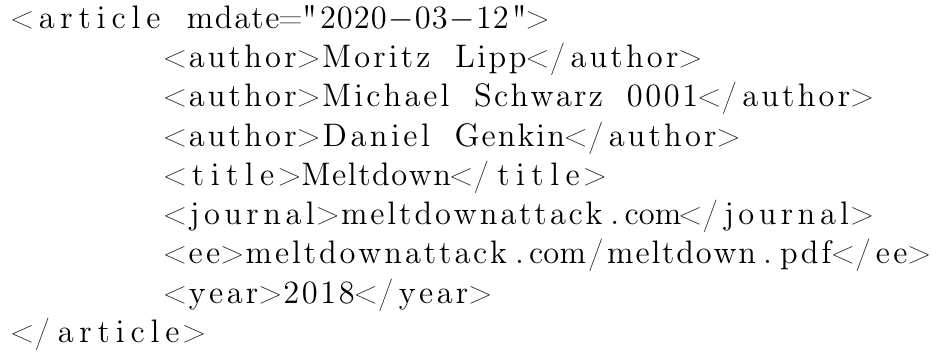
\includegraphics[width=14cm,keepaspectratio]{bilder/xmlAusschnitt}
	\caption{XML-Ausschnitt}
	\label{fig:xmlausschnitt}
	Ein Beispiel Ausschnitt wie ein typischer Eintrag in der dblp.xml aussieht. Dieser wurde verkürzt und angepasst.
\end{figure}

Der Parser ist in einer eigenen Klasse. Um mit dem Parser zu beginnen, werden die Daten zeilenweise in der Klasse eingelesen, um das Problem mit der Dateigröße zu umgehen. Denn würde alles auf einmal eingelesen werden, würde der Speicher des Programms schnell voll werden und damit den Computer überlasten. Nun wird in den Zeilen nach den Tags gesucht. Ist ein Tag gefunden worden, wird dessen Name überprüft und reagiert mit einem bestimmten Fall. Durch das zeilenweise Einlesen ist dies allerdings kein richtiger Streamparser, denn dieser würde Zeichen für Zeichen einlesen, um die Datei zu parsen. 

Da durch die Dokumentation alle Tags bekannt sind, die in der Datei auftreten können, müssen nur acht Fälle behandelt werden. Somit haben wir nur acht Methoden, mit denen wir jeden Fall abdecken. Alle von denen arbeiten genau ein Element ab. Jede Methode liest weitere Zeilen und Daten ein, bis das Endtag des gewissen Elements, die Methode beendet. Das zählt natürlich auch für das dblp-Endtag, welchen den Parser beendet. Die in der Zeit eingelesenen Tags und Werte sind die Attribute des entsprechenden Elements, wie bspw. bei ‚article‘, bei dem es der Autor sein kann, der eingelesen wird. 









Die Daten werden nun in eine weitere Klasse übergeben. Diese Klasse ist der DBParser, in diesem die Daten nochmals angepasst werden. Da die erste Klasse die Daten aus der XML-Datei in Daten in das Programm wandelt, wird diese Klasse nun die Daten so anpassen, sodass sie für die Datenbank nutzbar werden. Um nachher die Datenbank ordentlich verwenden zu können, werden die acht Elemente in Entitäten gewandelt, die vorteilhafter für das Datenbankdesign sind. Entitäten sind Objekte oder Wesen, die in der Datenbank mit Attributen und Werten befüllt werden können. Diese Einteilung wird im weiteren Verlauf noch gezeigt und erläutert. 

Zum Schluss werden in der Insert Klasse die Daten nur noch in die Datenbank eingefügt. Somit sind alle Daten von einem Element so gespeichert, dass der Arbeitsspeicher erneut benutzt werden kann. Damit wird dafür gesorgt, dass nur ein Element gleichzeitig bearbeitet wird und kein Speicherüberlauf auftritt. 

 
\begin{figure}[!htb]
	\centering
	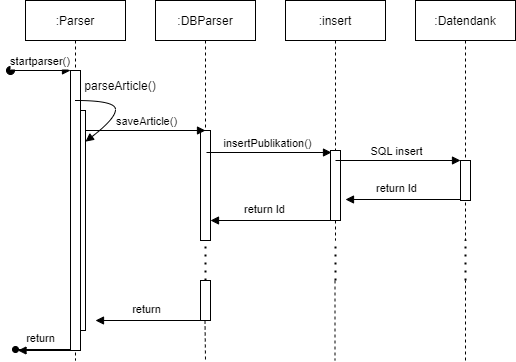
\includegraphics[width=15cm,keepaspectratio]{bilder/SequenzDiagramParser}
	\caption{Sequenzdiagramm-Auschnitt}
	\label{fig:sequenzdiagramm}
\end{figure}



Abbildung \ref{fig:sequenzdiagramm} zeigt einen typischen Programmverlauf eines Parsers. In diesem Beispielablauf wird ein ‚article‘ Element eingelesen. Zunächst wird die Parser-Klasse mit der startParser-Funktion in der Main-Methode aufgerufen und liest einen Tag nach dem anderen, bis er auf Treffer stößt. In diesem Fall ist das Tag ‚article‘ ein Treffer. Nun wird die parseArticle-Methode in der selben Klasse aufgerufen. In der Methode werden die darauffolgenden Elemente ausgelesen und deren Daten zwischengespeichert. Dies geschieht solange, bis das Endtag von ‚article‘ wieder eingelesen wird. Jetzt werden alle Daten an die saveArticle-Methode der DBParser-Klasse übergeben. In dieser Klasse werden nun die Daten an die Datenbank angepasst. Denn in dieser Datenbank gibt es keine Entität, die Artikel heißt. Das wird erst im nächsten Schritt erklärt. Im Allgemeinen wird der Artikel sowohl in Publikation, Autoren, elektronische Version und Fachzeitschrift als auch in die Beziehungen zwischen diesen Entitäten zerteilt. Da die Daten richtig zerlegt sind, werden sie an die Insert-Klasse einzeln übergeben. Das geschieht über die insertPublikation-Methode.


Jetzt sind alle Daten vorhanden und richtig zugewiesen. Daraufhin werden sie mit SQL in eine Postgres Datenbank gespeichert. Postgres ist ein freies objektrelationales Datenbankmanagementsystem (ORDBMS) und und basiert auf SQL.
SQL bedeutet Structured Query Language, also strukturierte Abfragesprache, und stellt einen Standard für relationale Datenbanken dar. Es gibt viele SQL-Datenbanken, wie zum Beispiel Amazon DynamoDB, IBM DB2, MongoDB, PostgresSQL u.Ä. 

PostgresSQL wird verwendet, da es sich zum einen um eine freie Oben-Source Datenbank handelt und zum anderen keine Lizenzen benötigt. Dazu hält sie weites gehend die SQL-Standards und Normen ein. Diese werden benötigt, um die Aufgabe ordentlich zu erfüllen. In den Methoden ist nämlich darauf zu achten, dass nur triviale SQL Befehle benutzt werden und keine speziellen eines bestimmten Datenbanktyps. Deshalb wird sich innerhalb dieser Arbeit auf Insert-Befehle und Select-Abfragen fokussiert, um auf keinen bestimmten Datenbanktypen angewiesen zu sein. 

Schlussendlich wird der Primärschlüssel der Publikation zurückgegeben, um die Beziehungen zwischen den Entitäten und der Datenbank einzutragen. Wenn nun die saveArticle-Methode zu Ende läuft und sich erfolgreich beendet, sucht die startparser-Methode nach dem nächsten Tag. So wird jedes Element nacheinander in die Datenbank eingespeichert, bis das Endtag von dblp eingelesen wird. 


\subsection{Datenbank}

Zur Erstellung der Datenbank werden zunächst die Daten analysiert. Die \textit{DBLP} gibt schon mit acht Elementen (article, inproceedings, proceedings, book, incollection, phdthesis, mastersthesis, www) einen groben Überblick. Diese Elemente sind allerdings noch nicht in dem relationalen Datenbankformat. Deshalb werden diese, wie vorhin erläutert, nochmal in kleinere Entitäten zerteilt. 
Für die Einteilung wird der \textit{Microsoft Graph} aus Abbildung \ref{fig:magschema} als Inspiration genommen, da bei dieser Zerkleinerung die Entitäten in ihrem fachlichen Kontext belassen werden müssen:

‚article‘ - Es setzt sich aus einer Fachzeitschrift, einer Publikation und mehreren elektronischen Versionen zusammen.

‚proceedings’ - Dies ist in diesem Zusammenhang eine Konferenz, die gehalten wurde
und besitzt Autoren, die diese Sammlung von Arbeiten angepasst haben. Diese Konferenz
kann auch ISBN’s enthalten.

‚inproceedings’ - Passend zu Konferenzen und ist eine Publikation, die in einer Konferenz veröffentlicht wurde.

‚book’ - Book ist ein Buch, mit ein oder mehreren Autoren. Hierzu gehören auch mehrere ISBN’s.

‚incollection’ - Dies sind Publikationen, die in einem Buch veröffentlicht wurden.

‚masterthesis’ - Die Masterthesis ist eine Publikation, die an einer Universität geschrieben wurde.

‚phdthesis’ - Im Gegensatz zur Masterthesis sind die phdthesis immer als Buch veröffentlicht.

‚www’ - Dies sind Homepages von Autoren, die abgegeben werden können.

Jede Publikation in den Erklärungen besitzt zusätzlich Autoren, die hier nicht aufgelistet sind. Dazu kommt noch, dass jeder Punkt elektronische Versionen enthält. Da in der \textit{DBLP} Bücher sind, die mehrere ISBN’s haben, muss eine extra Entität für die ISBN erstellt werden. Das Gleiche zählt für die elektronische Version, denn diese existiert für die meisten Entitäten mehrfach. Daraus ergeben sich dann diese Entitäten Autor, Publikation, Homepage, Konferenz, Fachzeitschrift, Buch, elektronische Version, ISBN und deren Beziehungen. Zu diesen Entitäten gehören ebenso die Attribute, die schon mit dem Parser eingelesen werden. Da nicht für jede Entität immer die gleiche Anzahl an Eigenschaften übergeben wird, werden die meisten Attribute optional. Mit den Entitäten und deren Attribute wird dann ein ER-Modell modelliert und an die entsprechenden Beziehungen angepasst.



\subsubsection{ER-Modell}
\begin{figure}[!htb]
	\centering
	\includegraphics[width=15cm,keepaspectratio]{bilder/ER-Modell}
	\caption{ER-Modell}
	\label{fig:er-modell}
\end{figure}


Das ER-Modell veranschaulicht die Beziehungen zwischen den Entitäten. Die Entitäten
sind hier die Rechtecke. Die Attribute sind Kreise und direkt mit den Entitäten verbunden, zu denen sie gehören. Beziehungen werden durch Rauten dargestellt und verbinden immer zwei Entitäten oder nur eine Entität mit sich selbst (siehe Beziehung hat-Zitat).
Ein Zitat verbindet eine Publikation, mit der Publikation, die zitiert wurde. Es wird deutlich, dass Beziehungen auch Attribute haben können, denn es gibt Fälle, wo dieses Attribut zu keinem von beiden passt. Das Attribut passt nur, wenn beide in Beziehung zueinander stehen. 
Die Relation zwischen Publikation und Buch besitzt sie das Attribut Seiten. Dies macht nur im einzelnen Zusammenhang Sinn, da Seiten allein in einer Publikation ohne Buch keinen Anhaltspunkt besitzen. Andersherum kann ein Buch mehrere Publikationen beinhalten und deshalb nicht verschiedene Seitenangaben für verschiedene Publikationen speichern. Somit macht die Angabe von Seiten nur in der Beziehung der beiden Entitäten Sinn. Mit Attributen werden Entitäten beschrieben und es gibt Attribute, die für eine eindeutige Identifikation der Entität sorgen. Diese Attribute
werden unterstrichen und nachher zu Schlüsselkandidaten. Die eindeutige Eigenschaft
bei Autor ist der Key. Dieser Key sieht wie in Abbildung \ref{fig:xmlausschnitt}. aus und ist der komplette Name eines Autors. Falls dieser Name doppelt vorkommt, haben die beiden Autoren eine zusätzliche Nummer hinter ihrem Namen. Dadurch wir dieser wieder ein Unikat.

Dieses Modell muss nun umgewandelt werden. Da in der Datenbank nur Tabellen angelegt werden können, muss dieses ER Modell in die Form von Tabellen gebracht werden. Diese Form ist dann das relationale Schema. Dieses Schema beschreibt genau das Gleiche, wie das ER-Modell, nur hier werden Fremdschlüssel und damit Beziehungen angegeben.


\subsubsection{Relationales Schema}

\begin{figure}[!htb]
	\centering
	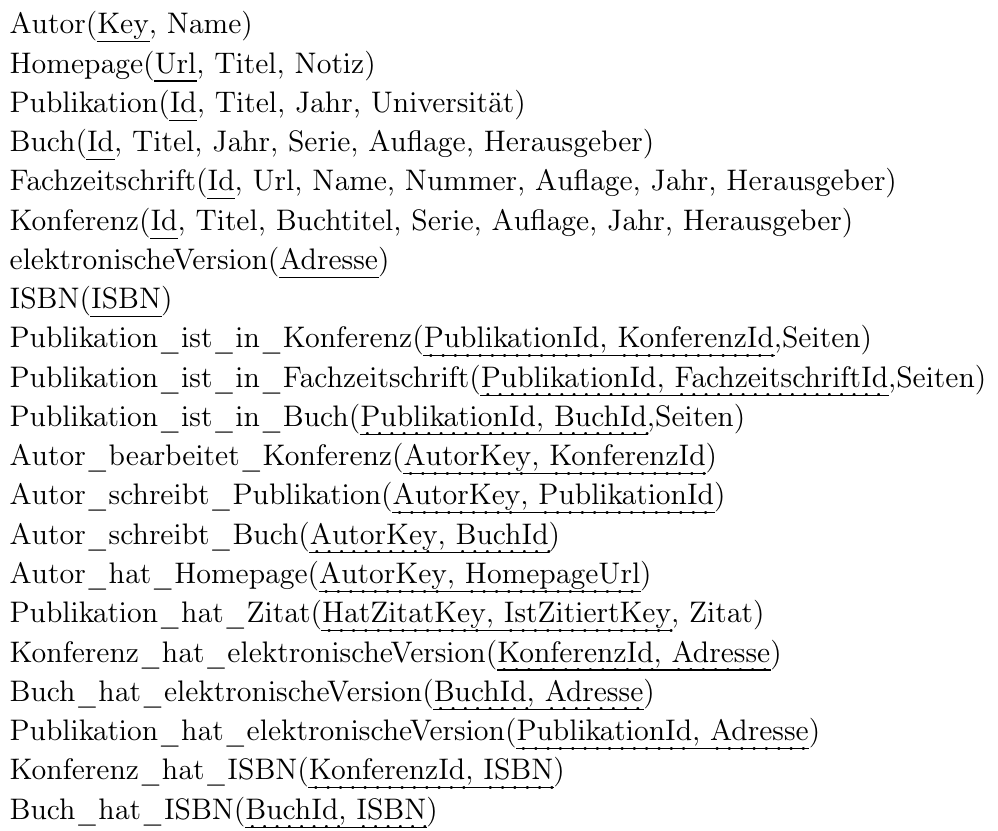
\includegraphics[width=12cm,keepaspectratio]{bilder/relationalesSchema}
	\caption{Relationales Schema}
	\label{fig:relationalesSchema}
\end{figure}


Abbildung \ref{fig:relationalesSchema} zeigt das ER-Modell, welches genau in das relationale Schema übertragen wurde. Der erste Name ist der Name der Tabelle und alle Namen in der Klammer sind deren Attribute. Es wird deutlich, dass auch Beziehungen zwischen den Entitäten eine eigene Tabelle bekommen. Diese sorgen dafür, dass Entitäten mit einander verbunden werden. Die unterstrichenen Attribute stellen die Primärschlüssel da. Primärschlüssel sind Attribute, womit die Daten dieser Entität genau unterscheiden werden können, wie bspw. die Studierendennummer, die sich bei jedem* Studenten* unterscheidet. Gibt es keine eindeutige Eigenschaft, so wird ein künstlicher Schlüssel erstellt. In diesem Fall heißen alle künstlichen
Schlüssel Id. Diese Id wird mit jeder Erstellung eines neuen Eintrags erhöht, damit
diese eindeutig bleibt. Die Attribute die mit Punkten unterstrichen wurden, sind Fremdschlüssel. Diese Schlüssel sind Primärschlüssel aus anderen Tabellen.
Um sich diese besser vorstellen zu können, wird ein Beispiel angeführt:

Es gibt 2 Entitäten, Schüler und Klasse. Der Primärschlüssel für die Klasse wäre die Klassen Bezeichnung, wie 2a oder 1b. Der Schüler hat eine Id als Primärschlüssel, da der Name nicht ganz eindeutig ist. Um nun die Relation so darzustellen, dass der Schüler in eine Klasse geht, wird den Klassen Schlüssel an die Schüler als Fremdschlüssel angefügt. Nun steht in der Schülertabelle bspw.:

Name: Max Mustermann und Klasse: 3a. 

Somit dient der Fremdschlüssel dafür dass Entitäten verbunden werden können.
Für das erste wird in dem Schema jede Beziehung als Tabelle mit zwei Fremdschlüsseln
erstellt. Die Schlüssel kommen aus den Entitäten, die sie verbinden. Damit stellen sie eine eindeutige Verbindung zwischen Entitäten her.

Da hier noch überflüssige Tabellen enthalten sind, werden die Tabellen verschmolzen.



\subsubsection{Verschmolzenes relationale Schema}

\begin{figure}[!htb]
	\centering
	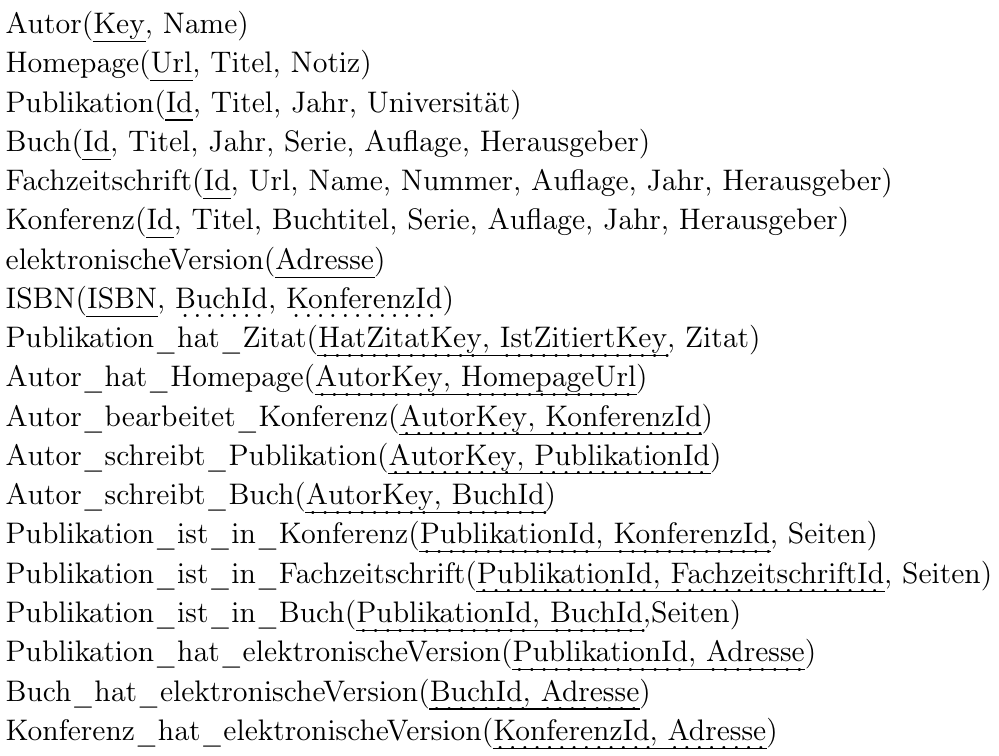
\includegraphics[width=13cm,keepaspectratio]{bilder/verschmolzenesRelationaleSchema}
	\caption{Verschmolzenes Relationale Schema}
	\label{fig:verschmolzenesrelationalesSchema}
\end{figure}






Abbildung \ref{fig:verschmolzenesrelationalesSchema} zeigt nun das verschmolzene relationale Schema. Einige Tabellen sehen jetzt anders aus. Zum Beispiel verschwindet die Tabelle Buch-hat-ISBN ganz, denn der Primärschlüssel vom Buch steht nun direkt in der ISBN, da es nur ein Buch für eine ISBN geben kann. Dasselbe passiert mit Konferenz und ISBN. Dies ist eine N zu 1 Beziehung gewesen, da Fälle auftreten, wo Bücher mehrere ISBN’s haben. Die meisten anderen Beziehungen sind N zu M Relationen, wie bspw. Autor und Publikation. Jeder Autor kann mehrere Publikationen schreiben und andersherum, denn Publikationen können von mehreren Autoren geschrieben werden. Diese Relationen können nicht verschmolzen werden. Der letzte Fall wäre eine 1 zu 1 Relation, aber die kommt in diesem Modell nicht vor. Ein typisches Beispiel ist eine Person und ihr Ausweis, denn eine Person hat nur einen Ausweis und ein Ausweis darf nur einer Person gehören.


\subsubsection{Normalisierung}

Normalisierungen sind dafür da, Fehler und Redundanzen zu verhindern. Redundanzen
sind doppelt oder mehrfach vorkommende Informationen. Diese können bei großen
Datenbanken für viel unnötigen Platzverbrauch sorgen. Fehler führen dazu, dass die Datenbank abstürzt oder Befehle verweigert werden. Die Normalisierung werden in Stufen von Normalformen getätigt.

Je höher die Stufe der Normalform, desto weniger Anomalien können auftreten. Anomalien sind die Ergebnisse von genau diesen Redundanzen, die denn Umgang mit der Datenbank erschweren oder sogar ganz stoppen. Es können Daten gelöscht werden, die noch gespeichert sein sollten. Werte und Datensätze können verschieden sein, die eigentlich gleich seien sollten. Insgesamt gibt es drei Anomalien, die einfach durch die Normalisierungen verhindert werden können.

Die Einfüge-Anomalie ist eine Anomalie, die beim Einfügen von Daten in der Datenbank
auftritt. Es kann passieren, dass ein Primärschlüssel aus zwei Schlüssel besteht.
Da das Einfügen nun verlangt, dass beide Primärschlüssel vorhanden sind, führt dies zu Schwierigkeiten oder auch zu Fehlern, wenn nur ein Teil vom Primärschlüssel
besessen wird. 

Beispiel:
\begin{figure}[!htb]
	\centering
	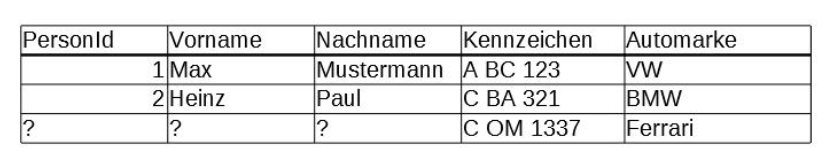
\includegraphics[width=13cm,keepaspectratio]{bilder/KFZBeispiel}
	\caption{Einfüge-Anomalie Beispiel}
	\label{fig:kfzbeispiel}
\end{figure}


Es wird davon ausgegangen, dass die Schlüssel PersonId und Kennzeichen zusammen den Primärschlüssel ergeben, da eine Person mehrere Autos haben kann. Soll jetzt ein neues Auto eingegeben werden, führt das zu Problemen, denn ein Auto kann in diesem Beispiel nicht ohne eine Person existieren. In Abbildung \ref{fig:kfzbeispiel} ist der Ferrari ohne Person und hat damit keinen vollständigen Primärschlüssel. Dies würde auch anderes herum zu Problemen führen, da eine Person auch nicht ohne ein Auto existieren kann. Somit haben wir eine Einfüge-Anomalie.

Die Änderungs-Anomalie tritt beim Ändern von Daten in der Datenbank auf. Wenn 
viele redundante Daten in einer Tabelle sind und ein Name geändert werden soll, tritt diese Anomalie auf, wenn dieser Namen an vielen Stellen geändert werden müsste - Wobei in diesem Fall eine Änderung reichen sollte.

Beispiel:
\begin{figure}[!htb]
	\centering
	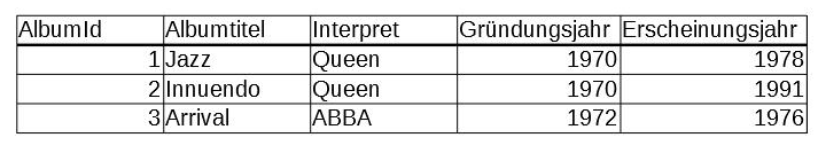
\includegraphics[width=13cm,keepaspectratio]{bilder/AlbumBeispiel}
	\caption{Lösch- und Änderungs-Anomalie Beispiel}
	\label{fig:albumbeispiel}
\end{figure}

Hier ist der Primärschlüssel die AlbumId. Die Probleme treten auf, wenn der Namen von Queen geändert werden würde. Normalerweise sollte eine Änderung reichen, um ein Attributwert zu ändern. In diesem Fall müsste jedes Album durchgegangen werden und da die Namen anpassen. Dieser extra Aufwand ist die Änderungs-Anomalie.

Die Lösch-Anomalie entsteht durch das Löschen von Daten aus der Datenbank.Wenn zwei unabhängige Daten gelöscht werden sollen und durch denn Aufbau beide Informationen gelöscht sind, entsteht eine Anomalie. Das Löschen sollte nur die Daten löschen, die auch beabsichtigt zu löschen sind. 

Beispiel aus Abbildung \ref{fig:albumbeispiel}:

Der Primärschlüssel ist immer noch AlbumId. Nun soll nichts mehr geändert, sondern gelöscht werden. Wenn jetzt das Album Arrival von ABBA gelöscht wird, würde damit auch direkt die Band ABBA gelöscht - obwohl nur beabsichtigt wurde, das Album zu löschen. 

Diese Anomalien werden alle durch die drei Normalformen beseitigt. 
Verschiedene Stufen der Normalformen sind:







Die erste Normalform besagt, dass jedes Attribut atomar sein soll. Damit ist gemeint, dass Daten zerkleinert werden sollen, die auch im einzelnen Aspekt eine Gewichtung haben, wie zum Beispiel Adressen. Adressen können als ein Ganzes zusammen geschrieben werden, aber Atomar wären sie erst, wenn sie in Straße, PLZ, Hausnummer und Stadt einteilt würden. Diese Einteilung verschafft nachher Vorteile, die für Datenbanken sinnvoll sind. Es kann einfacher nach Leuten gesucht werden, die alle in einer Stadt wohnen. Ohne diese atomaren Attribute müssten die Adressen für jede einzelne Suche zerlegen werden. Danach würde es erst möglich sein, die Städte zu vergleichen. Diese Regel wird leider in dieser Datenbank gebrochen, da die Namen von Autoren nicht in Vor- und Nachnamen geteilt sind.

In der DBLP sind die Autoren als ein ganzer Name gespeichert. Wären sie im Voraus getrennt gewesen, würden hier die Namen in Vor- und Nachname geteilt sein. Namen zu trennen ist eine Aufgabe für sich. Namen wie Jürgen von der Lippe oder Angela Dorothea Merkel haben schon verschiedene Trennungsmöglichkeiten. Hier ist zu sehen, dass es nicht einfach möglich ist, ab einer bestimmten Anzahl von schon eingelesenen Namen den Nachnamen zu bestimmen. Würde man den letzten Namen als Nachname festlegen, hat Jürgen von der Lippe nur einen Teil seines Nachname. Diese zu verallgemeinern, ist eine größere Aufgabe. Dazu kommen Namen aus Ostasien, die wiederum Vor-und Nachname andersherum aufschreiben, da der Familien Name zuerst genannt wird. Diese Aufteilung würde das Ausmaß dieser Arbeit überschreiten, sodass angenommen wird, dass Namen atomar sind. 

Für die zweite Normalform muss sie erst mal in der 1. Normalform sein und dazu darf kein Attribut, welches auch kein Primärschlüssel ist, eine Teilmenge in der Tabelle besitzen, die von dem Attribut abhängig ist. Demnach müssen Attribute vollständig von einem Primärschlüssel abhängig sein und nicht nur halb. Hierdurch wird auch die Einfüge-Anomalie gelöst, da es nun keine zwei einzelne Entitäten mehr gibt, die in eine Tabelle zusammen gefügt sind. Um dies zu verdeutlichen, wird erneut ein Beispiel angeführt:


\begin{small}
	Person(\uline{Id}, Name, Nachname, Kennzeichen, Automarke, Autotyp)
\end{small}


In dieser Tabelle wäre das Kennzeichen ein Primärschlüssel von einer Automarke und eines Autotyp und damit hat ein Nichtprimärattribut eine Teilmenge von Attributen, die von ihm abhängig ist. Zwar gehört das Auto dieser Person, aber es wäre nur vollständig abhängig von der Kombination der beiden Attribute Id und Kennzeichen. Damit ist diese Tabelle nicht in der zweiten Normalform, denn dafür müssen die Tabellen so aussehen:

\begin{small}
	Person(\uline{Id}, Name, Nachname, \dotuline{Kennzeichen})\newline
	Auto(\uline{Kennzeichen}, Automarke, Autotyp)
\end{small}


Für die dritte Normalform muss zunächst die Tabelle in der zweiten Normalform sein und dann darf kein Nichtprimärschlüssel transitiv von einem Schlüsselkandidaten abhängen. Schlüsselkandidaten sind Attribute, die als Primärschlüssel Infrage kommen. Durch diese Normalform werden direkt zwei Anomalien beseitigt, die Änderung-Anomalie und die Lösch-Anomalie. 

Um dies zu verdeutlichen, ein weiteres Beispiel:

\begin{small}
	Album(\uline{Id}, Albumtitel, Interpret, Gründungsjahr, Erscheinungsjahr)
\end{small}


Hier wäre das Gründungsjahr transitiv über Interpret abhängig, denn Gründungsjahr wäre erst über den Interpreten mit dem Album verlinkt und würde somit die Regel brechen. Demnach muss der Interpret eine eigene Entität werden. Damit sehen die Tabellen dann so aus:

\begin{small}
	Album(\uline{Id}, Albumtitel, Erscheinungsjahr, Interpret)\newline
	Künstler(\uline{Interpret}, Gründungsjahr)
\end{small}


Die Tabelle ist in der dritten Normalform, wenn man davon ausgeht, dass der Interpret eindeutig ist, ansonsten wird noch ein künstlicher Schlüssel eingefügt. 

In der dritten Normalform sind nun alle Anomalien beseitigt. Das sind die Grundeigenschaften, die eine Datenbank erfüllen muss. Diese Datenbank erfüllt alle Kriterien der dritten Normalform, wenn davon ausgegangen wird, dass Namen ungetrennt schon atomar sind, falls nicht wären sie in der nullten Normalform.


\newpage
\subsection{Datendefinition in der Datenbank}


Nun wurde der gesamte theoretische Teil dieser Datenbank beschrieben. Für die Praxis wird SQL verwendet, bei dem es sich um eine Datensprache handelt. Sie ist dafür da, Datenbanken zu erstellen und zu verwalten. Diese Sprache teilt sich in drei Hauptteile von Befehlsgruppen ein, DDL für die Struktur der Datenbank, DML für das Daten manipulieren und DQL für das auslesen der Daten. Diese drei Teile werden benötigt und noch im weiteren Verlauf erklärt.

Hierzu wird DDL - \textit{ausgeschrieben Data Definition Language} - verwendet. Diese Sprache wird benutzt, um die Datenstruktur, die theoretisch aufgebaut wurde, in der Datenbank anzulegen. Also alle Tabellen, Beziehungen, Datentypen u.Ä.


\begin{figure}[!htb]
	\oranget{CREATE TABLE} AUTORSCHREIBTBUCH( \newline
	KEY \purplet{VARCHAR(100)} \oranget{NOT NULL},\newline
	ID \purplet{INTEGER}        \oranget{NOT NULL},\newline
	\oranget{PRIMARY KEY}(KEY,ID),\newline
	\oranget{FOREIGN KEY}(KEY) \oranget{REFERENCES} AUTOR(KEY)\newline
	\oranget{ON DELETE} CASCADE \oranget{ON UPDATE} CASCADE,\newline
	\oranget{FOREIGN KEY}(ID) \oranget{REFERENCES} BUCH(ID)\newline
	\oranget{ON DELETE} CASCADE \oranget{ON UPDATE} CASCADE);\newline
	\caption{DDL Ausschnitt}
	\label{fig:ddlbeispiel}
\end{figure}


Abbildung \ref{fig:ddlbeispiel} zeigt einen typischen SQL Auschnitt, in der die Tabelle Autor-schreibt-Buch erstellt wird. Dabei ist zu beachten, dass SQL nicht case sensitive ist, also achtet die Sprache nicht auf Groß- und Kleinschreibung. Wie hier zu sehen ist, wird erst der Create-Befehl benutzt, sodass eine Tabelle namens AUTORSCHREIBTBUCH erstellt wird und in der dahinterliegenden Klammer die Tabellenstruktur kommt. Hier werden erst die beiden Attribute Key und ID erstellt. Hinter den jeweiligen Namen kommen die Datentypen in Varchar und Integer. Varchar steht für eine variable Zeichenkette mit einem Maximum an Zeichen. Variabel ist sie, da sie nicht immer die maximale Anzahl als Speicher einnimmt. Integer steht für eine Ganzzahl. Fasst alle Attribute sind in Varchar gespeichert, da die DBLP nicht genormt ist. Viele Werte, die eigentlich ein Integer wären, werden durch Ausnahmen wieder zu Varchar, bspw. gibt es bei Büchern das Attribut Auflage(Volume). Durchweg werden hier Ganzzahlen verwendet, die Auflagen beschreiben, aber manche Auflagen sind mit langen komplizierten Zeichenketten beschrieben, was Integer wieder hinfällig macht. Deshalb sind nur die künstlichen Schlüssel vom Typ Integer. Diese Tabelle ist die Relation zwischen Autor und Buch. Deshalb sind beide Attribute Fremdschlüssel(Foreign Key). Erst wird der Fremdschlüssel als ein solcher markiert und danach wird dieser auf die Tabelle mit dem Attribut, zu dem es gehört, referenziert. Dabei spielt es keine Rolle, ob der Fremdschlüssel denselben Namen hat wie der Primärschlüssel, den er repräsentiert. So könnte auch der Fremdschlüssel umbenannt werden und im Nachhinein trotzdem auf den richtigen Primärschlüssel verweisen. Es könnte zum Beispiel ID auf BuchId geändert werden, wozu nur die zwei ID’s umbenannt werden, aber dabei nicht die Referenz geändert muss.

Unter dem Foreign-Key-Befehl stehen noch optionale Eigenschaften zu Fremdschlüsseln. Hiermit wird beschrieben, was bei einer Änderung oder Löschung von dem Primärschlüssel in der referenzierten Tabelle passiert. Es gibt fünf Möglichkeiten, die eingestellt werden können:

NO ACTION - Hier wird nichts mit der Tabelle getan. Da dann aber ein Fremdschlüssel
auf einen Datensatz verweist, wird ein Fehler geworfen. Dies ist auch die Standardeinstellung, wenn keine Option gewählt wurde.

RESTRICT - Es wird verboten, den verwiesenen Primärschlüssel zu löschen.

CASSCADE - Der Tabelleneintrag wird gelöscht/geändert, falls der verwiesene Primärschlüssel gelöscht wird oder sich ändert.

SET NULL - Der Fremdschlüssel wird auf Null gesetzt, wenn der verwiesene Primärschlüssel gelöscht wird oder sich ändert.

SET DEFAULT - Wie bei SET NULL, nur hier wird der Fremdschlüssel auf den voreingestellten Standardwert gesetzt.

In diesem Fall werden beide Male CASSCADE benutzt, da dies eine Relationstabelle ist und diese die Änderungen und Löschungen mit übernehmen soll. Da diese Tabelle nur die Beziehung darstellt und keine wirklichen Daten besitzt, geschehen hiermit keine Löschungen oder Änderungen, die Fehler erzeugen könnten.


\subsection{Daten einfügen}

Nun wird die Datenbank, mit den Daten die schon mit dem DBParser angepasst wurden, befüllt. Hierfür wird Data Manipulation Language (DML) verwendet, also die Datenbearbeitungssprache, welche wieder einen Teil von SQL darstellt. Mit diesem Teil können Daten eingefügt, geändert oder auch gelöscht werden. In diesem Teil der Arbeit wird die Hauptaufgabe das Einfügen sein.

\begin{figure}[!htb]
	%\includegraphics[width=13cm,keepaspectratio]{bilder/DDLBeispiel}
	\oranget{INSERT INTO} AUTOR (KEY, NAME)\newline
	\oranget{VALUES} (???,???);\newline
	\caption{DML Ausschnitt}
	\label{fig:dmlbeispiel}
\end{figure}

In Abbildung \ref{fig:dmlbeispiel} wird ein Datensatz in die Autor-Tabelle eingetragen. Mit dem INSERT INTO Befehl wird bestimmt, dass Daten eingespeist werden sollen. Nach dem INTO kommt die Tabelle in welche gespeichert wird. In der Klammer sind dann die Attribute angegeben, die bei diesem Datensatz befüllt werden sollen. Hinter VALUES in der Klammer werden nun die Daten in der Reihenfolge eingefügt, wie sie in der ersten Klammer schon angegeben wurden, ein. Die Fragezeichen stellen in diesem Beispiel die Daten da. Da der Key ein Primärschlüssel ist, tritt ein Fehler auf, wenn zwei Mal der gleiche Wert dafür einfügt wird. Dadurch wird klar, dass der Datensatz schon vorhanden ist.













\newpage
\section{Erweiterung}




In diesem Abschnitt geht es hauptsächlich um die Erweiterung der Datenbank. Erst wird die richtige Methode ausgewählt, mit der die Daten geholt werden. Dann werden die Informationen über die Zitate abgerufen und nachher in die Datenbank eingefügt.

Für die Erweiterung wird der \textit{Microsoft Academic Knowledge Graph}(siehe \cite{DBLP:conf/semweb/Farber19}) benutzt, da dieser im Gegensatz zur \textit{DBLP} zusätzliche Zitate hat und diese, um die entsprechenden Zitate, erweitert werden können.

Es existieren wieder zwei Möglichkeiten, an die Daten zu kommen, eine API und ein Dump File. Das Dump File wurde seit 2018 nicht mehr aktualisiert,trotzdem hat die Summe aller Daten des Dump Files 1,2 Terabyte. Da mit diesem Teil nur die bestehende Datenbank erweitert werden soll, lohnt es sich nicht, eine Datenbank runter zuladen, die viel größer ist als diese. Da nur nach Zitaten gesucht wird, lohnt sich die Vorgehensweise mit den Dump Files nicht. 

Deswegen wird hier das \textit{Project Academic Knowledge} verwendet. In diesem Projekt gibt es die \textit{Academic Search API}. (siehe \cite{PAK} ) Also eine Schnittstelle, mit der in dem Graph gesucht und Daten ausgelesen werden können. Es werden vier verschiedene REST API’s zur Verfügung gestellt: CalcHistogram, Interpret, Similarity und Evaluate.



CalcHistogram - Hier werden alle Suchergebnisse zusammen gerechnet und ein Histogramm darüber erstellt. Dabei kann eine Häufigkeitsverteilung über alle Attributswerte von den gesuchten Publikationen erhalten werden.(vlg. \cite{PAKAPI})

Interpret - Diese Schnittstelle funktioniert wie eine automatische Vervollständigung und gibt Lösungsvorschläge an. Dies kann am besten nach jeder Zeicheneingabe abgefragt werden.(vlg. \cite{PAKAPI})

Similarity - Dies gibt die Möglichkeit, zwei verschiedene Publikationen auf Gleichheit zu prüfen. Die Rückgabe ist eine Gleitkommazahl die von +1.0, sehr ähnlich bis zu -1.0 sehr unähnlich reicht.(vlg. \cite{PAKAPI})

Evaluate - Mit Evaluate können normale Suchanfragen gestellt werden und es wird eine Menge von akademischen Entitäten zurückgegeben, die dazu passen.(vlg. \cite{PAKAPI})


In dem Fall wird Evaluate verwendet, da weder ein Histogramm, noch einen Vergleich oder eine automatische Vervollständigung gebraucht wird. Bei dieser Anfrage können bestimmte Suchkriterien selber eingestellt werden. Dafür muss ein vorgegebenes Suchattribut mit einem Suchwert verglichen werden. Hier kann zum Beispiel als Attribute Name des Autors ausgewählt werden, wo dann der Suchwert den Namen des zu suchenden Autors enthält. Für diese Attribute gibt es eine ganze Dokumentation.


Ein paar Beispiele werden später benannt. Wird nichts weiteres angegeben, werden alle Informationen über die gesuchte Entität ausgegeben. Um diese Ausgabe zu verringern, werden bei der Suche weitere Optionen angegeben, mit der die Ausgabe angepasst wird. Hier können Optionen gewählt werden wie count, um die Anzahl der Ergebnisse anzupassen, offset, um nicht die ersten Ergebnisse ausgegeben zu bekommen, orderby, um nach einem Attribute zu sortieren oder attributes, um nur bestimmte Attribute auszugeben.


\begin{figure}[!htb]
	\centering
	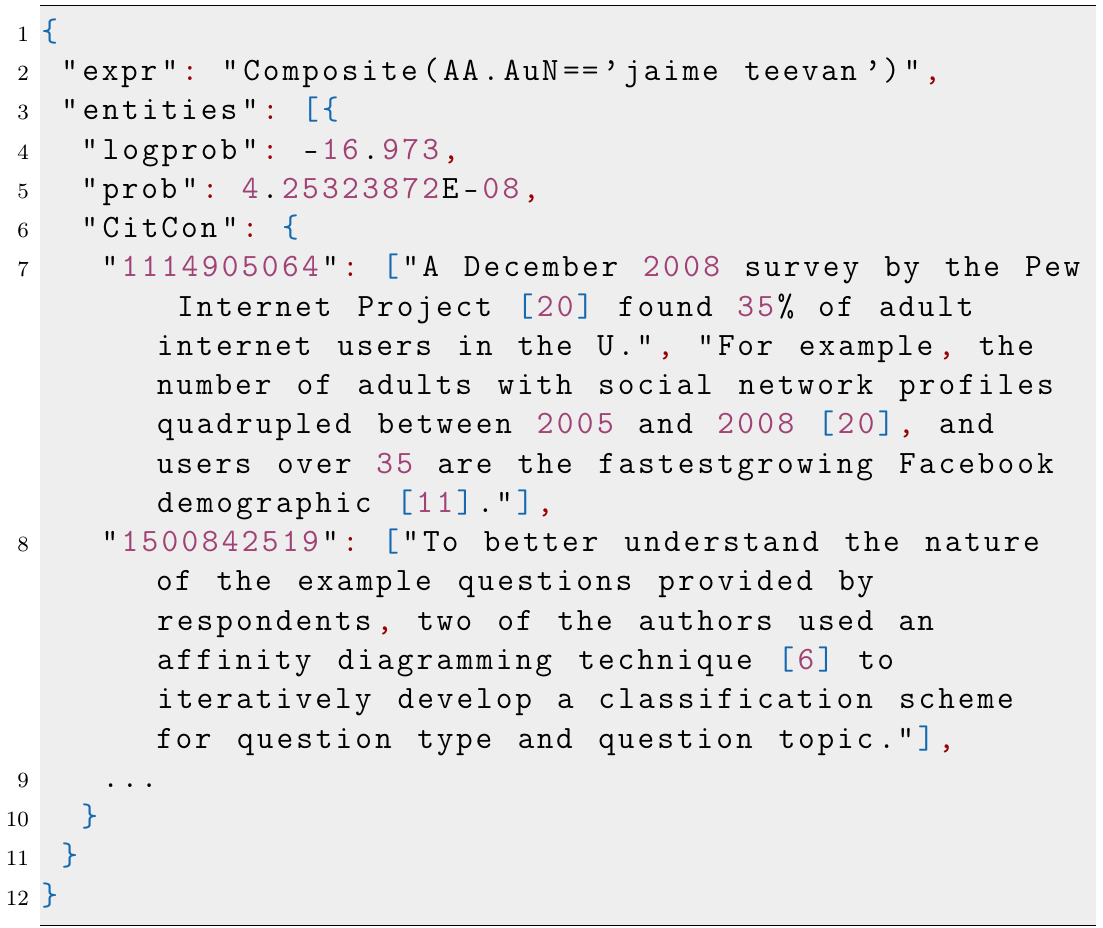
\includegraphics[width=12cm,keepaspectratio]{bilder/ResponseBeispiel}
	\caption{Response Beispiel}
	\label{fig:response-beispiel}
\end{figure}



Die Response aus Abbildung \ref{fig:response-beispiel} ist im JSON-Format. Diese dient genau wie XML für die Speicherung von menschlich lesbaren Daten.(vlg \cite{json}) Der gezeigte Ausdruck ist ein Beispiel, in dem nach einem Autor namens ’jaime teevan’ gesucht wird. Die Ausgabe der Attribute wurde nur auf ’CitCon’ beschränkt. Dies ist das Attribute für Zitate. Dennoch werden ’logprob’ und ’prob’ hinzugefügt. Da die Responses sehr kurz sein werden, müssen keine Parser selbst geschrieben werden. Somit kann ein fertiger Parser benutzen werden, der die Daten heraus filtert. Nun muss die Anfrage gesendet werden. 

Mit dieser relativ simplen API kommt aber auch eine Grenze. Es muss ein kostenloses Abonnement abgeschlossen werden, um Zugriff zu erhalten. Dafür ist ein an den Account gebundener Schlüssel nötig, mit dem die API benutzt werden kann. Im Monat dürfen mit diesem Schlüssel nur 10.000 Transaktionen getätigt werden. Durch diese Einschränkung werden hier nur selektive Beispiele präsentiert. Deshalb wird hier eine Funktion genutzt, die die ersten 200 Publikationen ausgibt. Mit diesen 200 Daten wird das Erweitern getestet und begutachtet.

Zunächst werden aus der Datenbank 200 Titel heraus genommen. Diese 200 Titel werden nun einzeln angepasst, um sie mit einer Request loszuschicken, denn die API kann keine Sonderzeichen oder Großschreibung verwenden. Nachdem die ganze Punktierung entfernt und kleingeschrieben wurde, wird die Anfrage mit der Bedingung geschickt, dass ‚Ti’ gleich des angepasstem Titel sein soll. ‚Ti’ steht für normalized title. Dieser Titel ist auch klein geschrieben und ohne Sonderzeichen. Damit werden schnell passende Publikationen gefunden. Mit der Filtereinstellung ‚CitCon’ kann nun die Id und der Abschnitt, der zitiert wurde, erhalten werden.



Nun wird eine Antwort erhalten wie in Abbildung \ref{fig:response-beispiel}. Daraufhin werden die wichtigen Informationen mit Hilfe eines Standard JSON-Parsers herausgefiltert. Falls der Titel kein Zitat besitzt, wird der Titel übersprungen und der nächste Titel angefragt. Wenn doch ein Zitat zu diesem Titel gefunden wurde, sind die relevanten Daten in der Antwort. Diese sind die Paper Id und das Zitat an sich. 

Die Paper Id ist in dieser Datenbank nicht zu gebrauchen, da diese nur zu den Publikationen in dem Microsoft Graphen gehören. Deswegen muss diese Id in etwas umwandeln werden, mit dem gearbeitet werden kann. In diesem Fall ist das wieder ein Titel. Für die Umwandlung wird eine weitere Anfrage an die Schnittstelle gestellt. Diese sucht nach Publikationen mit der selben ID, sodass der Titel zurückgegeben wird. Da die API nur Probleme bei der Eingabe von Sonderzeichen hat, aber nicht bei der Ausgabe,wird der Titel mit Sonderzeichen und Großschreibung zurückgegeben. Dazu wird der Filterwert  ‚DN’ verwendet, der den originalen Titel liefert. 

Somit sind alle Daten vorhanden, die gebraucht werden, um ein Zitat in die Datenbank einzuspeisen. Zunächst gibt es den Titel, wofür die Zitate gesucht wurden. Dann wurde ein das Zitat mit der Paper Id von der zitierten Publikation erhalten. Schlussendlich wurde daraus auch der Titel der Publikation erhalten. Nun muss nur noch der Titel in unserer Datenbank gefunden werden um die PublikationsId zu erhalten. Denn in unserer Relation, mit der die Zitierung dargestellt wird, werden die beiden Primärschlüssel der Publikationen benötigt. Es kann passieren das die Id von der Zitierten Publikation nicht in unserer Datenbank gefunden wird, da im Academic Graph mehr Werke gespeichert sind als in unserer und dadurch sich nicht alle Arbeiten überschneiden. Wurden die Daten gefunden, werden sie einfach mit einem DML-Befehl in die Datenbank eingefügt. 

So wird die Datenbank Schritt für Schritt erweitert. 






\section{Ergebnis}
Schluss endlich haben wir eine uns mit Python eine Datenbank aufgebaut. Dies haben wir mit erst mit der Planung und dann mit der Ausführung bewältigt. Zu nächst haben wir uns die Daten angeguckt. Dann haben wir daraus ein ER-Modell erstellt und dies in ein relationales Schema gebracht. Dieses Schema haben wir dann verschmolzen um die letzte theoretische Übersicht der Datenbank aufzuzeigen. Darauf hin haben wir uns Anomalien angeguckt und Normalformen um diese zu verhindern. Danach haben wir uns die eigentliche Erstellung der Datenbank angeguckt und wie man mit SQL eine Tabelle einfügt. Nun haben wir die Daten nur noch eingefügt und abgespeichert. 

Dieses Einfügen klappt mit einer Geschwindigkeit von 40-60 Transaktionen die Sekunde, dass heißt nur für grob 5 Millionen Publikationen würden wir 100.000 Sekunden brauchen das sind 1667 Minuten oder auch ca. 28 Stunden. Davon abgesehen das noch 2 Millionen Autoren da zu kommen. Dazu kommt noch das Transaktionen nicht nicht Publikationen pro Sekunde sind, denn in Publikationen sind alleine zwischen 2-4 Autoren beteiligt die jedes mal Abgefragt werden müssen ob sie Existieren und wenn nicht angelegt werden. Hier müssen natürlich auch die Relationen angelegt werden die die beiden Tabellen verbindet. Daraus werden dann pro Publikation dann mindestens 6 Transaktionen mehr. Dazu kommen noch die ein bis zwei elektronischen Versionen pro Publikation mit den Relationen. Somit landen wir grob bei einer Dauer von 308 Stunden das sind fasst 13 Tage. Da durch viele erneute Anpassungen der Datenbank dieser Prozess wiederholt werden musste, werden hier nur Ausschnitte der bisherigen Ergebnisse gezeigt. 

Dazu verwenden wir Data Querie Language(DQL) eine Datenabfragesprache die wieder ein Teil von SQL da stellt. Hiermit können wir Anfragen an die Datenbank stellen die uns dann dem entsprechende Antworten liefert. Mit diesem Teil von SQL kann in der Datenbank nichts geändert werden weder Struktur noch Daten.

\begin{figure}[!htb]
	\centering
	%\includegraphics[width=14cm,keepaspectratio]{ER-Modell}
	\caption{DQL Beispiel}
	\label{fig:dqlbeispiel}
\end{figure}

Erklärung...%todo

\begin{figure}[!htb]
	\centering
	%\includegraphics[width=14cm,keepaspectratio]{ER-Modell}
	\caption{DQL Ergebnis}
	\label{fig:dqlergebnis}
\end{figure}
\section{Ausblick}
%todo

%%%%%%%%%%%%%%%%%%%%%%%%%%%%%%%%%%%%%%%%%%%%%%%%%%%%%%%%%%%%%%%%%%%%%%%%
%%%% ENDE TEXTTEIL %%%%%%%%%%%%%%%%%%%%%%%%%%%%%%%%%%%%%%%%%%%%%%%%%%%%%
%%%%%%%%%%%%%%%%%%%%%%%%%%%%%%%%%%%%%%%%%%%%%%%%%%%%%%%%%%%%%%%%%%%%%%%%

\clearpage

% Entfernen Sie das Kommentar aus der nachfolgenden Zeile, falls Sie einen Anhang in der Arbeit verwenden wollen. Beachten Sie, dass Sie sich im Verlauf der Arbeit mit \ref{...} (z.B. \ref{anhang:zusatz1}) auf den Anhang beziehen.
%\newpage
\appendix
\section{Anhang}

\subsection*{Zusatzteil 1} \label{anhang:zusatz1}

Dies ist ein Anhang.

\clearpage

\ifthenelse{\boolean{\biber}}{ %with biber do
	\DeclareNameAlias{sortname}{first-last}
	\printbibliography[heading=bibintoc, title=\references]
}{ %without biber do
	\bibliography{references}
	\bibliographystyle{alphadin}
}
%\vspace*{\fill}

\clearpage

\listoffigures

\listoftables

%\pagebreak

%\printindex
\end{document}
